\documentclass[11pt,a4paper]{article}

\usepackage[margin=1in]{geometry}
\usepackage{amsmath, amssymb}
\usepackage{graphicx}
\usepackage{tikz}
\usetikzlibrary{arrows.meta}
\usepackage{hyperref}
\usepackage{listings}
\usepackage{booktabs}
\usepackage{longtable}
\usepackage{xcolor}
\usepackage{framed}
\usepackage{float}
\usepackage[skip=1em]{parskip}

\lstset{
  basicstyle=\ttfamily\small,
  breaklines=true,
  frame=single,
  showstringspaces=false,
}

% Inline code. Usable in math mode, where \texttt alone would be ignored.
\newcommand{\fn}[1]{\ifmmode\text{\ttfamily #1}\else\texttt{#1}\fi}

\newenvironment{warningbox}%
  {\par\begin{framed}\noindent\textbf{Note.}\ \ignorespaces}%
  {\end{framed}\par}

\title{Debugging Playbook for Ultrasound Segmentation}
\author{Dale Kernot}
\date{\today}

\begin{document}
\maketitle
\tableofcontents

\newpage
\section{Purpose}
This note records a practical workflow for finding and isolating failures in
the segmentation pipeline. Cases often run to completion without crashing, so
visual inspection of batch HTML is the primary way to spot errors. Once a bad
case is identified, a single-image run with targeted debug plots is used to
test a hypothesis about where the pipeline went wrong.

Functions named without a module prefix live in \fn{general\_functions.py}.
The batch entry point is \fn{python -m usseg.main}. The single-image entry
point is \fn{data\_from\_image}, exercised by
\fn{tests/single\_image\_processing\_test.py}.

\section{Debugging loop}
\label{sec:loop}

\begin{figure}[H]
\centering
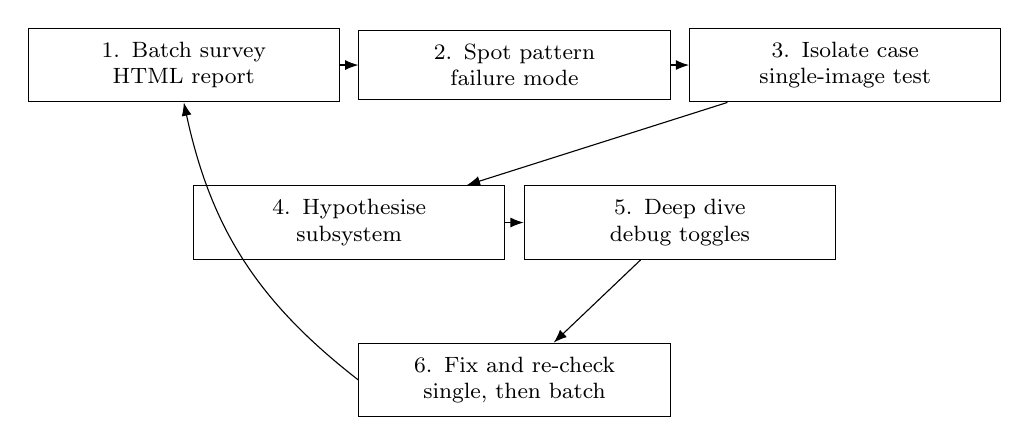
\begin{tikzpicture}[
  font=\footnotesize,
  >=Latex,
  box/.style={draw, align=center, inner sep=5pt, text width=3.6cm},
]
  \node[box] (batch) at (0,0)
    {1. Batch survey\\HTML report};
  \node[box] (pattern) at (4.2,0)
    {2. Spot pattern\\failure mode};
  \node[box] (isolate) at (8.4,0)
    {3. Isolate case\\single-image test};
  \node[box] (hyp) at (2.1,-2.0)
    {4. Hypothesise\\subsystem};
  \node[box] (dive) at (6.3,-2.0)
    {5. Deep dive\\debug toggles};
  \node[box] (fix) at (4.2,-4.0)
    {6. Fix and re-check\\single, then batch};

  \draw[->] (batch) -- (pattern);
  \draw[->] (pattern) -- (isolate);
  \draw[->] (isolate) -- (hyp);
  \draw[->] (hyp) -- (dive);
  \draw[->] (dive) -- (fix);
  \draw[->] (fix.west) to[bend left=20] (batch.south);
\end{tikzpicture}
\caption{High-level debugging loop. Batch HTML finds patterns; single-image
runs confirm the failing subsystem.}
\label{fig:loop}
\end{figure}

\subsection{Step 1: batch survey}
Configure \fn{config.toml} (\fn{root\_dir}, \fn{output\_dir}) and run from the
repository root with the project environment active:

\begin{lstlisting}
python -m usseg.main
\end{lstlisting}

This finds candidate images, segments them, writes pickles and intermediate
figures under \fn{output\_dir}, and produces
\fn{generated\_segmented\_data.html} in the working directory. Open the HTML
and scan for systematic problems: wrong scale, bad envelopes, missing
digitised metrics, doubled mean waves, and so on.

\begin{warningbox}
Batch mode is deliberately quiet on debug figures. Do not rely on the
\fn{SHOW\_*} toggles during a full run; they are for single-image
investigation.
\end{warningbox}

\subsection{Step 2: spot a pattern}
Ask whether the failure is isolated or shared across the dataset. Shared
failures often point to a method or calibration assumption (for example
right-axis ticks on a particular scanner layout). Isolated failures may be
image quality, unusual annotation layout, or a single bad segmentation seed.

Record for each suspect case:
\begin{itemize}
  \item source image path (from the HTML row / output prefix),
  \item which HTML columns look wrong (annotated, digitised, mean wave, table),
  \item which model looks best or worst (ray / morph / grow), if relevant.
\end{itemize}

\subsection{Step 3: isolate the case}
Copy the failing path into
\fn{tests/single\_image\_processing\_test.py} and run:

\begin{lstlisting}
python tests/single_image_processing_test.py
\end{lstlisting}

This calls \fn{data\_from\_image} on one file and plots the returned trace. A
clean exit does \emph{not} mean the result is correct: the same silent
inaccuracies seen in HTML can appear here. Use the batch hypothesis to decide
what to inspect next.

\subsection{Step 4: hypothesise from the HTML}
Use the visible HTML columns as a coarse fault tree. Envelope shape is decided
before beat metrics; axis calibration is decided before digitised $y$ values
make sense. Table~\ref{tab:symptoms} summarises common mappings.

\subsection{Step 5: deep dive with toggles}
Near the top of \fn{general\_functions.py} (around lines 277--285) are module
flags that enable intermediate matplotlib figures:

\begin{lstlisting}
SHOW_BEAT_DEBUG_SUBPLOTS = False
SHOW_GROW_DEBUG_PLOTS   = False
SHOW_MORPH_DEBUG_PLOTS  = False
SHOW_RAY_DEBUG_PLOTS    = False
SHOW_TICK_LABEL_DEBUG_PLOTS = False
\end{lstlisting}

Turn on only the flag(s) for the suspected subsystem, re-run the single-image
test, and inspect the windows. Leave batch flags off again before the next
full \fn{main} run.

\subsection{Step 6: fix and re-check}
Confirm on the single image first, then re-run a small batch or the full
\fn{main} HTML to check that the fix did not regress other cases.

\section{Symptom to subsystem map}
\label{sec:symptoms}

\begin{longtable}{@{}p{0.34\textwidth}p{0.32\textwidth}p{0.28\textwidth}@{}}
\caption{HTML / visual symptoms mapped to likely code areas and debug
entry points.}
\label{tab:symptoms}\\
\toprule
What you see & Likely area & Start here \\
\midrule
\endfirsthead
\toprule
What you see & Likely area & Start here \\
\midrule
\endhead
\bottomrule
\endfoot
Axis scale wrong; digitised $y$
  systematically high/low &
Tick / label finding; axis
  calibration &
  \fn{search\_for\_ticks},
  \fn{search\_for\_labels},
  \fn{validate\_axis\_ticks};
  \fn{SHOW\_TICK\_LABEL\_DEBUG\_PLOTS} \\
\addlinespace
Envelope shape wrong for one
  method &
That segmentation method &
\fn{SHOW\_MORPH\_DEBUG\_PLOTS},
  \fn{SHOW\_RAY\_DEBUG\_PLOTS},
  or \fn{SHOW\_GROW\_DEBUG\_PLOTS} \\
\addlinespace
Envelope looks OK; PS/ED or feet
  wrong; doubled / empty mean wave &
Beat / foot detection &
\fn{SHOW\_BEAT\_DEBUG\_SUBPLOTS};
  also \fn{mean\_wave} /
  \fn{\_beat\_detection\_pass\_feet} \\
\addlinespace
OCR values present; digitised
  columns empty or all red &
\fn{plot\_correction} fill, or
  beat detection failed for that
  series &
Logs + beat debug; check
  peaks/troughs on figure~2 \\
\addlinespace
Crash, missing table, or blank
  HTML row &
Earlier stage: text OCR, coarse
  ROI, axes &
\fn{batch\_main.log}; single-image
  traceback; \fn{initial\_segmentation} \\
\end{longtable}

\section{Existing debug toggles}
\label{sec:toggles}

These flags live in \fn{general\_functions.py}. When any of them is true,
\fn{data\_from\_image} keeps matplotlib figures open
(\fn{\_maybe\_close\_figures} skips \fn{plt.close("all")}).

\begin{description}
  \item[\fn{SHOW\_MORPH\_DEBUG\_PLOTS}]
    Morphological refine stages and Method~1 envelope overlays.
  \item[\fn{SHOW\_RAY\_DEBUG\_PLOTS}]
    Ray-tracing main steps (clustering, yellow exclusion, picks, smooth).
  \item[\fn{SHOW\_GROW\_DEBUG\_PLOTS}]
    Region-grow main steps (seed, yellow forbid, grown mask, envelope).
  \item[\fn{SHOW\_BEAT\_DEBUG\_SUBPLOTS}]
    Beat / foot overlays and derivative / search-window panels inside
    \fn{plot\_correction}.
  \item[\fn{SHOW\_TICK\_LABEL\_DEBUG\_PLOTS}]
    Axis tick and label search: thresholded ROI, right-axis tick-object
    filter, column-score profile, retained tick contours, and OCR label
    boxes matched to tick centres (\fn{search\_for\_ticks} /
    \fn{search\_for\_labels}).
\end{description}

\begin{warningbox}
Leave these flags \fn{False} for batch \fn{main} runs. Enable only the
subsystem under investigation for single-image debugging.
\end{warningbox}

\section{Command cheat sheet}
\label{sec:commands}

Batch HTML (repo root, venv active):
\begin{lstlisting}
python -m usseg.main
\end{lstlisting}

HTML only, from an existing \fn{segmented\_data.pkl}:
\begin{lstlisting}
python -m usseg.visualisation_html
\end{lstlisting}

Single-image investigation:
\begin{lstlisting}
# edit img_path in tests/single_image_processing_test.py
python tests/single_image_processing_test.py
\end{lstlisting}

Logs from a direct \fn{main} run are appended to \fn{batch\_main.log}. Profiler
dumps from \fn{main}'s \fn{prof} wrapper are written as
\fn{get\_likely\_us.log}, \fn{segment.log}, and
\fn{generate\_html\_from\_pkl.log}.

\section{Open improvements}
\label{sec:open}

Useful next steps for this playbook / tooling (not yet implemented):
\begin{itemize}
  \item Move \fn{SHOW\_*} flags into a \fn{[debug]} section of \fn{config.toml}
    so investigation does not require editing source.
  \item Make each HTML row show the full source path (and a ready-to-paste
    single-image command) to shorten the batch$\to$isolate step.
  \item Optionally record a short case log template (path, symptom, hypothesis,
    toggle used, outcome) for recurring failure modes.
\end{itemize}

\end{document}
